\section{The news browsing problem}
\label{sec:newsgraph}

Our problem statement can be formally stated as:
\begin{quote}
  Create an end-to-end news browsing system which given a
  continuous stream of raw news articles, processes these articles to
  mine and track the underlying news stories and visualizes these for
  a user on an easy-to-use, queryable, personalized and context-full
  interface.
\end{quote}
As discussed in the previous section, various approaches have been proposed in the past to tackle one or more components of the above problem
statement. In this section, we first define a notion of contextuality of a browsing system, and motivate the need for the system to serve multiple flexible and personalizable contexts to a user as per her
requirements and/or preferences. We reason why we think this is a necessary feature of a news browsing system. Next, we show how rich contexts can be served to a user on the fly based on her intent
from the graph structure created from the input news corpus, taking specific examples. 
Finally, we describe some other desirable features of a news browsing tool. 

\subsection{Context in News browsing}
Let us attempt to define clearly what we mean by context. The
dictionary definition of the word is ``the circumstances that form the
setting for an event, statement or idea, and in terms of which it can
be fully understood and assessed.'' But the term ``circumstances'' is
vague and does not help us. So, instead, viewing the news corpus as a
time indexed set, we can think of the following definition: 
\begin{quote}
Given a news article or articles {\em context} is that set of stories
preceding, co-occuring or following that article or articles which
enhance our understanding of the events or ideas described in that
article or articles.
\end{quote}

Context for a user using our system, comprises of articles, topics,
actors, events, etc which though not directly related to particular
story, helps to interpret the story in a broader sense.  Adding
context serves to make it easier for users to better understand chain
of news articles around an event. For eg., consider a crime story
where the prime suspect is $X$. To fully understand the involvement of $X$ in the story,
one may be required to go through articles which would have first reported the crime (and not 
mentioned $X$). These articles serve as context. Hence, one way to think of context-serving articles
are \emph{articles which are coherent with articles containing $X$ and have still more information to provide.}

Given this intuition, we now propose a natural algorithm to determine useful context for a particular part of
the news graph in consideration. We first define the notion of Continue strength $\Omega$ of an actor at some time.
Let $\Lambda$ be the set of all actors, $T$ the time index set,
and $\Omega : \Lambda \times T \rightarrow [0,1]$ gives an actor's continue strength at some time. This score is
aggregated over all the articles featuring this actor.
\begin{equation}
\Omega(\lambda, \tau) = \frac{\sum_{a \in A([\tau - P, \tau + F])}{ContinueScore(\lambda, a)}}{|\{a  | a \in A([\tau - P, \tau + F])\}|}
\end{equation}
Here, $ContinueScore(\lambda, a)$ is the continue score (as defined in \cite{choudhary@ecir2008}) of an actor $\lambda$ occurring in article $a$ published around the current time point $\tau$. This score is
normalized between 0 to 1. $P$ and $F$ are past and future time windows that we keep at 50 days each, and $A([\tau - P, \tau + F])$ are all the articles in this time window.

Given an article $a$, we define $coh_{a}(b)$ as the \emph{coherence} between $a$ and some another article $b$. Intuitively, coherence captures the continuity of story when the two articles are read in succession.
Clearly, coherence between 2 articles depends on the amount of their actor/topic overlap. Moreover, common actors with strong continue scores contribute less to coherence. So, we quantify coherence as
\begin{equation}
coh_{a}(b) = \frac{\sum_{\lambda \in E(a) \cap E(b)}{\Omega(\lambda, \tau)^{-1}}}{|E(a) \cup E(b)|}
\end{equation}
where $E(a)$ is the set of actors occurring in article $a$ and $\tau$ is the time at which article $a$ is published. 

Along the same lines, we define $cont_{a}(b)$ as the \emph{context} given by article $b$ to $a$. There are primarily two different kinds of context: a) Context of different actors/topics and how they lead
to the story in A and b) Context of the same actors/topics in a slightly different setting. Context added by article $b$ can be quantified by the degree of ``new information'' added by $b$. So, we evaluate
context as
\begin{equation}
cont_{a}(b) = \frac{\sum_{\lambda \in E(b)}{\Omega(\lambda, \tau)*ContinueScore(\lambda, a)^{k}}}{|E(b) - E(a)|}
\end{equation}
where $k \in [-0.5, 0.5]$ is a user-input parameter which influences which of the 2 kinds of context is more prominent. A higher $k$ prefers context having more information
around the same actors as those of our article of interest.

A context-giving article is only useful as long as it is coherent with the original article(s).
Hence, we have to combine these 2 metrics. Before this, we normalize both these metrics to 0 to 1.
Finally, we apply the following algorithm to get the ``most useful'' neighbourhood of a result set of article nodes.

\begin{algorithmic}
  \State \textbf{procudure GetNeighbourhood:}
  \State \algorithmicrequire{Node $n$, Current Weight $w$, Threshold $\theta$}
  \State \algorithmicensure{Neighbourhood $N$}
    \If {$w < \theta$}
      \State return
    \EndIf
    \ForAll{node $v \in E(n)$}
      \If {! visited($v$)} 
        \State visited($v$) = True
        \State $w_1 = coh_{n}(v)$
        \State $w_2 = cont_{n}(v)$
        \State $w_3 = w_{(n,v)}$
        \State GetNeighbourhood($n, w_1 * w_2 * w_3, \theta$)
      \EndIf
    \EndFor
\end{algorithmic}

Through this algorithm, we look are assured of a good context coverage while keeping the coherence high.
An important point to note here is that all of these scores need only by computed once and stored, and not computed for every user query. 

We now give some examples of context in the news graph.
\begin{figure}
\caption{Robert Vadra corruption story and its contexts}
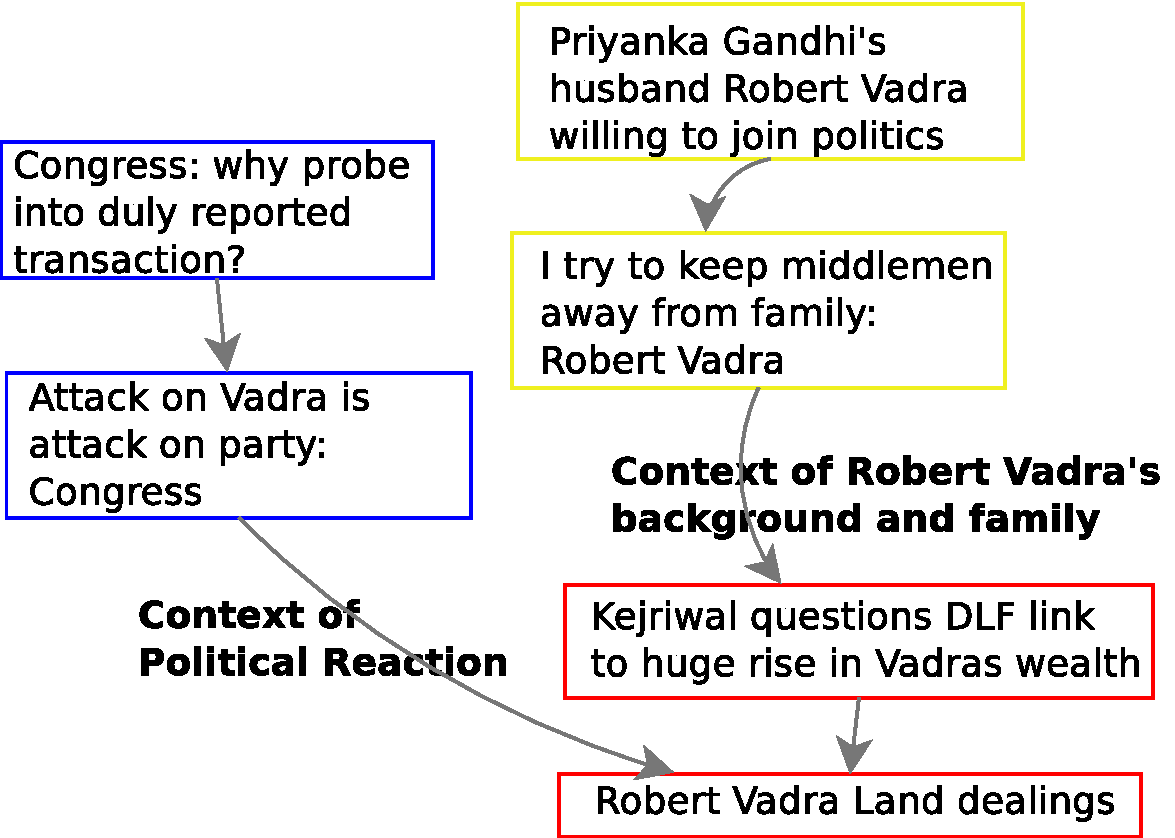
\includegraphics[scale=0.36]{figures/graph-vadra.pdf}
\label{fig:vadra-corruption}
\end{figure}

Consider Figure~\ref{fig:vadra-corruption} showing the graph of the story around Robert Vadra's alleged
corruption scandal reported in the news. As the story progresses in time, the articles
start to assume that the reader has enough knowledge of who Robert Vadra is, what is he known for,
how has this controversy spiralled to include the top political parties of India, etc. Hence, these articles
become increasingly inaccessible to a user with less prior context. However, 
using the graph, we can provide this context at any stage. Moreover, while following the story, 
the reader can look for how have the political parties reacted to this story as another context.

\begin{figure}
\caption{The fuel price hike story (September 2012) and its contexts}
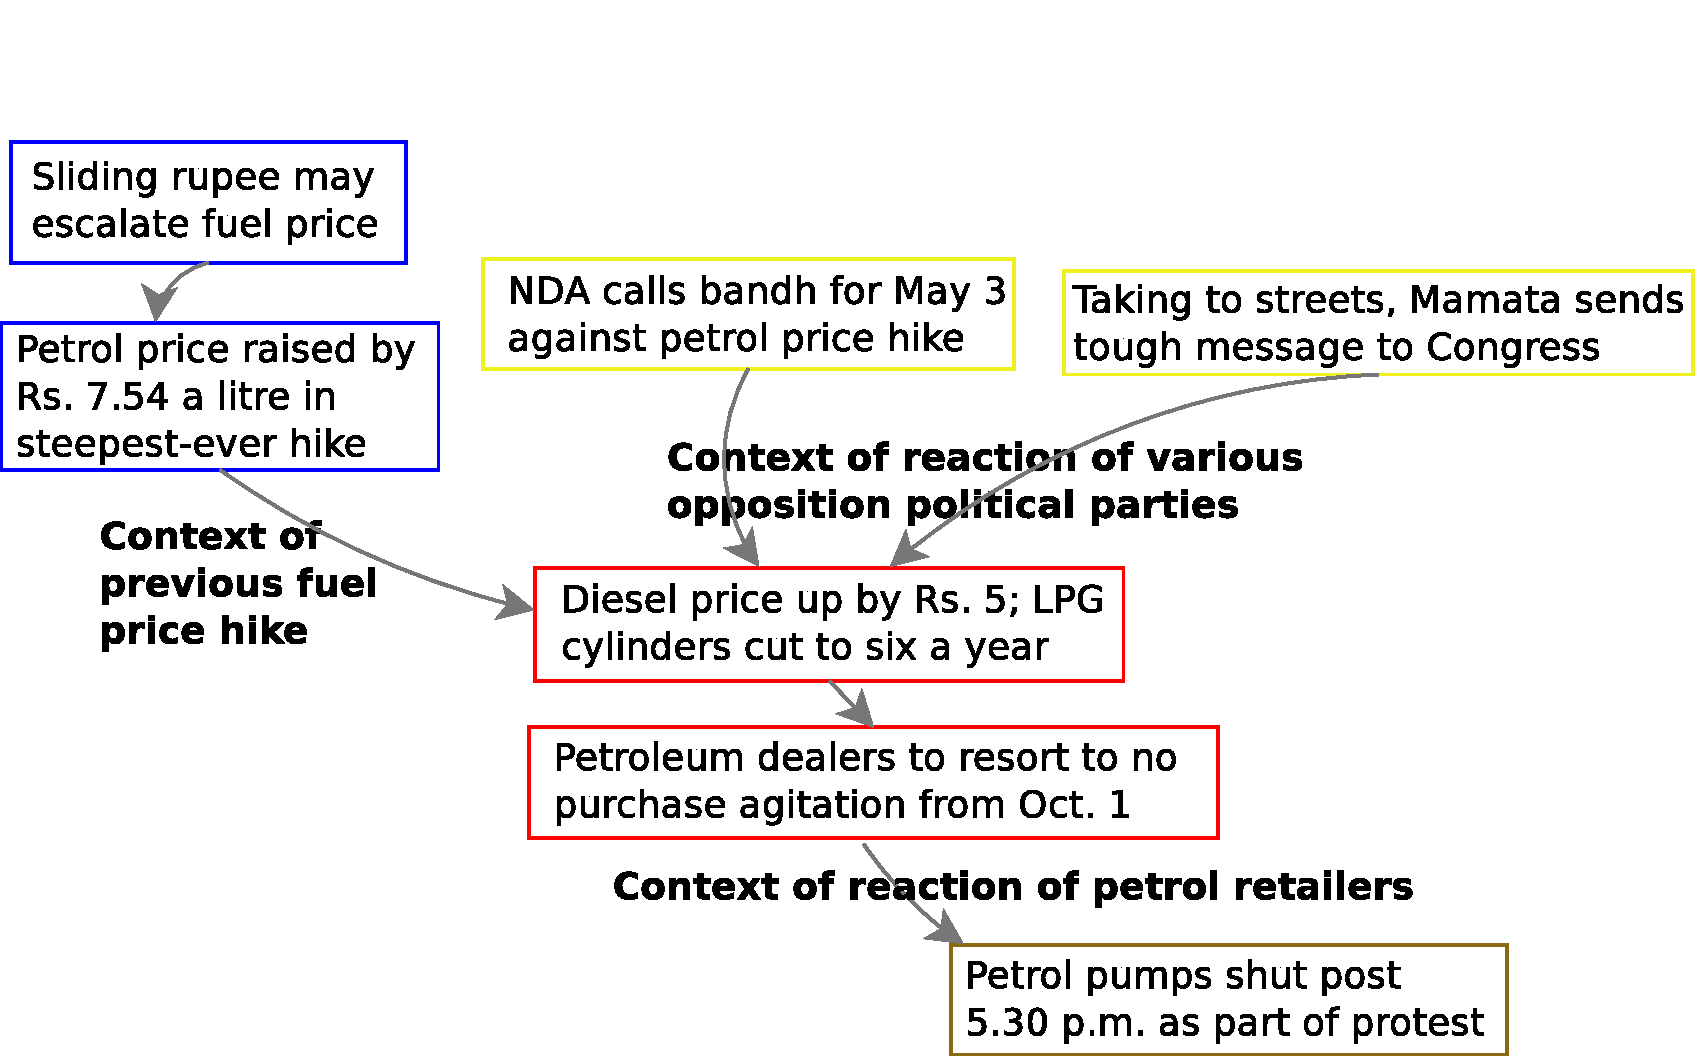
\includegraphics[scale=0.32]{figures/graph-petrol.pdf}
\label{fig:petrol}
\end{figure}

As a final example, consider the Figure~\ref{fig:petrol} showing the graph of the articles talking
about the Indian government's decision to raise the fuel price, and its past and subsequent developments. 
For a user wanting to deeply understand the circumstances behind fuel price hikes in India, the context of 
all past fuel price hikes is vital. For other users, the political
sphere and its reactions or the reactions of the petrol retailers may be of more interest.

As we have seen context is a fairly general notion and can be
instantiated in many ways depending on the user's point of view. It is
also clear from the examples above that the primary mode of inferring
contextual relationships between articles is by studying the
co-occurence and development of relationships of actors and topics in
time. We now discuss the {\em news graph} first defined
in~\cite{choudhary@ecir2008}, which provides a natural representation
of such relationships.


\subsection{How the news graph of~\cite{choudhary@ecir2008} creates personalized contexts}
Using the graph, the users have access to multiple contexts which
develop a unique aspect of the story they are following, and which
could highlight and bring forth previously unknown connections among
actors and topics. In this section, we will take examples to show how
different users would want/choose to explore same/different contexts
of the same story they are studying.

Consider two different users, both of whom want to study the Delhi gang-rape story visualized in Figure~\ref{fig:context-adding-graph-gang-rape-1}. However, when presented
one of the users wishes to study the reactions of politicians in depth, while the other wants to analyze the response and effectiveness of the police
machinery. Both these users will focus on different contexts, and soon personalize the base graph by filtering on it appropriate to their information
requirement. As a system, we never took any rigid decision to call only some of the related nodes as the ``most appropriate context''. This allows
the user to look through multiple other contexts, and then have the flexibility to choose the one that interests them the most. Moreover, this context
is calculated on the fly subject what part of the graph is in focus at that instant. As the users move across in the graph, the contexts for them keep
changing, and we can track these contexts efficiently using the graph structure.

Consider Figure~\ref{fig:context-graph-example} where 3 distinct stories are presented. The nodes marked $A$(in blue) cover a case involving Dominique Strauss-Kahn (DSK), 
those marked $B$(in red) cover of a case surrounding Pascal Mazurier(PM), and those marked $C$(in green) talk of the internationally reported Gang-rape case
that happened in Delhi(DGR).\footnote{Kindly note that in no way do we want to use this unfortunate incident or others used in the paper in any way except 
to exemplify the technicalities of our work. As reported in \cite{subasic-icdm:2008}, it is unfortunate that negative incidents are highlighted in the media
with greater vociferousness.} Two key things can be noted here. Even with a fair overlap of topics (Sexual Assault, Rape), the DSK and DGR subgraphs are not directly linked to each other.
On the other hand, the PM and DSK stories have a direct link in between them. This points to the fact, that the graph algorithm is successfully able
to determine how close or far stories (subgraphs) are to each other. Moreover, for any subgraph, one can define the \emph{context-giving node} as 
a neighbour which when shown to the user, would make it easier for her to understand the story and put in a broader perspective. For eg., if someone
wants to know about Ram Singh, the prime accused in the DGR case, just looking at the articles featuring Ram Singh won't suffice, since he would be
discussed in other articles where his name won't have featured explicitly (as he is still on the run). Such context-giving nodes are shown in bold outline in the figure.

Figure~\ref{fig:sample-news-graph} shows an example graph that gets created for a set of 4
articles covering a crime story. Nodes $A$ and $B$ talk about the incident being reported, reactions from various sections of the society and
the progress of investigation. Then, there is a fork in the story, with node $C$ talking about the fate of the investigating officer Damayanti Sen, 
and node $D$ talks covers the judicial probe of the incident. The nodes $C$ and $D$ cover different different aspects of the same story. 
\begin{figure}
\caption{A news graph of a crime incident from Bengal}
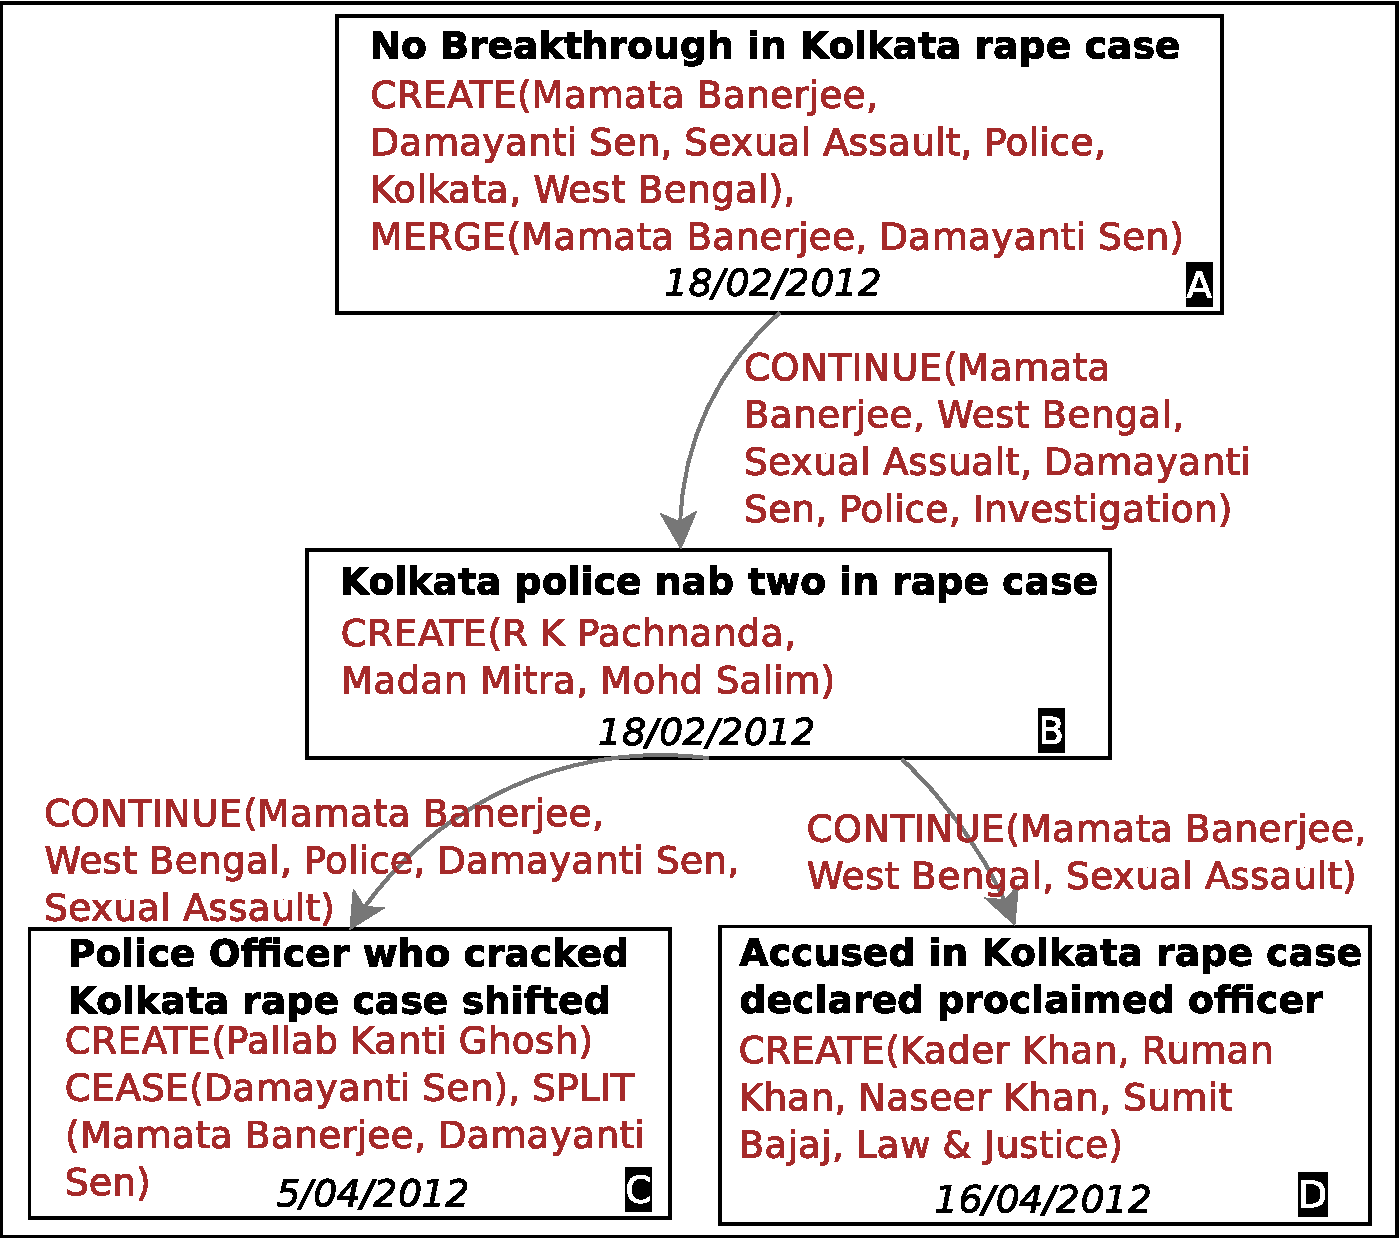
\includegraphics[scale=0.36]{figures/graph-1.pdf}
\label{fig:sample-news-graph}
\end{figure}
A key strength of our approach is that we allow the user to iteratively query the underlying corpus on multiple parameters and never have to recreate
the graph. Having created the graph once, we just filter out only the relevant nodes clusters and visualize them on a timeline as events. 
On searching for specific actors, we look at the node clusters containing these actors and visualize those clusters. This helps put those actors
in a broader context. For eg., looking for convicts in a particular crime story, would return not just the story of their judicial probe, but of
the whole case connected through other actors and topics.

